\documentclass{beamer}
\usepackage[T1]{fontenc}
\usepackage[utf8]{inputenc}
\usepackage{hyperref}
\usepackage{graphicx}
\usepackage{caption}
\usepackage{listings}
\usepackage{color}
\usepackage{verbatim}

%\usecolortheme{wolverine}
\usetheme{Madrid}



\AtBeginSection[]
{
    \begin{frame}
        \author{}
        \subtitle{}
        \title{\insertsection}
        \date{}
        \maketitle
        
    \end{frame}
      
    \begin{frame}
        % \frametitle{\insertsection}
        % \tableofcontents[currentsection]

        % Make a table of contents with only the current section showing the next subsections
        \frametitle{\insertsection}
        \tableofcontents[currentsection, hideothersubsections]

    \end{frame}
}


% Define the textttcolor --> blue marine
\definecolor{textttcolor}{RGB}{0, 102, 204}

% Set the default color for \texttt{}
\let\oldtexttt\texttt
\renewcommand{\texttt}[1]{\textcolor{textttcolor}{\oldtexttt{#1}}}


\title[Cloud Computing final project]{\Huge{Cloud Computing final project}}
\subtitle{A cloud-based file storage system \\ and the OSU benchmarks in k8s}
\author{Isac Pasianotto}
\date{2023-02-12}



\begin{document}

\begin{frame}
    \titlepage
\end{frame}

\section{Cloud \textbf{basic} module}
\subsection{Requirements}

\begin{frame}
    \frametitle{Requirements}
    things must be placed there
\end{frame}

\subsection{Nextcloud: the chosen solution}
\begin{frame}
    \frametitle{Nextcloud: the chosen solution}
    User and admin features, ...
\end{frame}

\begin{frame}
    \frametitle{Nextcloud: the chosen solution (cont.)}
    security, ...
    encryption, ...
\end{frame}

\subsection{Deployed structure}
\begin{frame}
    \frametitle{Deployed structure}
    \begin{figure}
        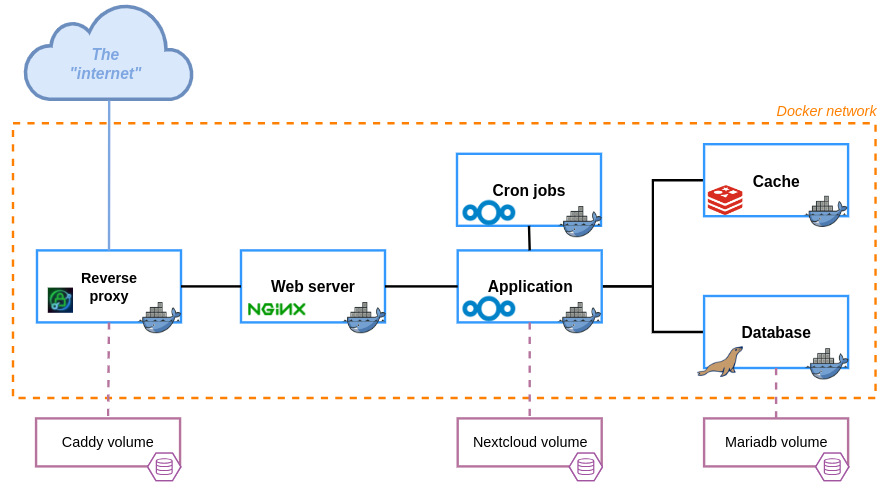
\includegraphics[width=\textwidth]{images/other/exbasediagram}
        %\caption{Description of the deployed structure}
    \end{figure}
\end{frame}

\subsection{Load test: Locust}
\begin{frame}
    \frametitle{Load test: Locust}
    How it was done, ...
\end{frame}

\begin{frame}
    \frametitle{Load test: Locust (cont.)}
    Results, ...
\end{frame}

\subsection{Scalability}
\begin{frame}
    \frametitle{Scalability}
    How can it be done, ...
\end{frame}

\begin{frame}
    \frametitle{Scalability (cont.)}
    Pro and cons of various solutions, ...
\end{frame}


\section{Cloud \textbf{basic} module: Nextcloud in a kubernetes flavor}

\subsection{Different architecture}
\begin{frame}
    \frametitle{Different architecture}
    What is different, ...
\end{frame}

\begin{frame}
    \frametitle{Different architecture (cont.)}
    \begin{figure}
        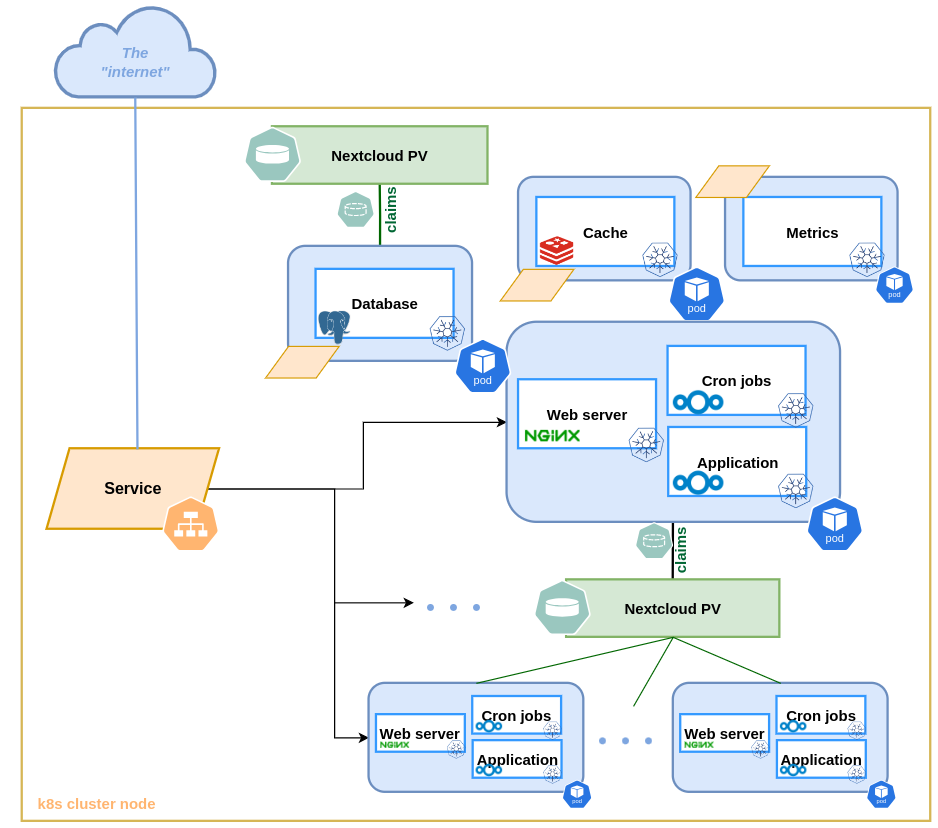
\includegraphics[height=0.85\textheight]{images/other/exadvanceddiagram}
        %\caption{Description of the deployed structure}
    \end{figure}
\end{frame}

\subsection{How to deploy}
\begin{frame}
    \frametitle{How to deploy}
    The magic of helm
\end{frame}

\subsection{Benefits of kubernetes}
\begin{frame}
    \frametitle{Benefits of kubernetes}
    What are the benefits, ...
\end{frame}

\section{OSU benchmarks in k8s}
\subsection{What are the OSU benchmarks}
\begin{frame}
    \frametitle{What are the OSU benchmarks}
    What are the OSU benchmarks, ...
\end{frame}

% ...

\end{document}